A key goal of our parallel design is to keep the threads as busy as possible and
to reduce inter-thread communication. Initially, the VM will partition the
application graph of $N$ nodes into $T$ subgraphs (the number of threads) and
then each thread will work on their own subgraph. Reduction of communication
between nodes in different threads is achieved by compiler as explained before
and the threads only need to initialize their pre-defined sub-graphs.

During execution, threads can steal nodes of other threads to keep themselves
busy. The load balancing aspect of the system is performed by our work scheduler
that is based on a simple work stealing algorithm. The pseudo-code for the main
thread loop is shown in Fig.~\ref{alg:thread_work_loop}. In each round, a thread
inspects its work queue for active nodes with new candidate rules and, if there
is any, procedure \texttt{process\_node()} executes it. If the work queue is
empty, the thread attempts to steal half of the nodes from another thread.
Starting from a random thread, it cycles through all the threads to find one
active thread. Eventually, there will be no more work to do and the threads will
go idle. There is a global atomic counter, a global boolean flag and one state
flag for each thread that are used to detect termination. Once a thread goes
idle, it decrements the global counter and changes its flag to idle. If the
counter reaches zero, the global flag is set to idle. Since every thread will be
busy-waiting and checking the global flag, they will detect the change and stop
executing.

\begin{figure}
\begin{algorithm}[H]
   \KwData{Thread TH, THREADS}
   \While{true}{
      $node \longleftarrow TH.work\_queue.pop\_node()$ \;
      \uIf{$node$}{
         $TH.process\_node(node)$\;
      }
      \Else{
         \tcc{Need to steal some nodes.}
         $target \longleftarrow random(len(THREADS))$\;
         $i \longleftarrow 0$\;
         \For{$i < len(THREADS)$}{
            $target \longleftarrow (target + 1) \% len(THREADS)$\;
            $nodes = THREADS[target].steal\_half()$\;
            \If{$len(nodes) > 0$}{
               $TH.work\_queue.add\_to\_queue(nodes)$\;
               break\;
            }
            $i \longleftarrow i + 1$\;
         }
         \If{$len(TH.work\_queue) == 0$}{
            \tcc{try to terminate}
            $TH.become\_idle()$\;
            \If{$TH.synchronize\_termination()$}{
               \Return{}\;
            }
            \tcc{There's new nodes in the queue.}
            $TH.become\_active()$\;
         }
      }
 }
\end{algorithm}
\caption{Thread work loop: threads process active nodes from the work queue
   until no more active nodes are avaiable. Node stealing using a \emph{steal
      half} strategy is employed when the thread has no more active nodes.}
 \label{alg:thread_work_loop}
\end{figure}

Figure~\ref{fig:implementation:vm_overview} presents the layout of our virtual
machine for a program with six nodes and two running threads. Each thread space
includes the nodes owned by the thread (the dotted arrows represent the edges
between nodes) and a \emph{Work Queue}, which contains \emph{active nodes},
i.e., nodes that have new facts to process, and can be implemented as a simple
linked list. Initially, the \emph{Work Queue} is filled with all the nodes of
the thread in order to derive the axioms.
Figure~\ref{fig:implementation:vm_overview} also illustrates the internal
structure layout of a node, which includes: the database of linear facts
(\emph{Linear DB}); the database of persistent facts (\emph{Persistent DB}); the
rule matching structures (\emph{Rule Engine}); and an auxiliary buffer for
storing intermediate facts coming from other threads (\emph{Fact Buffer}).

\begin{figure*}[t]
\centering
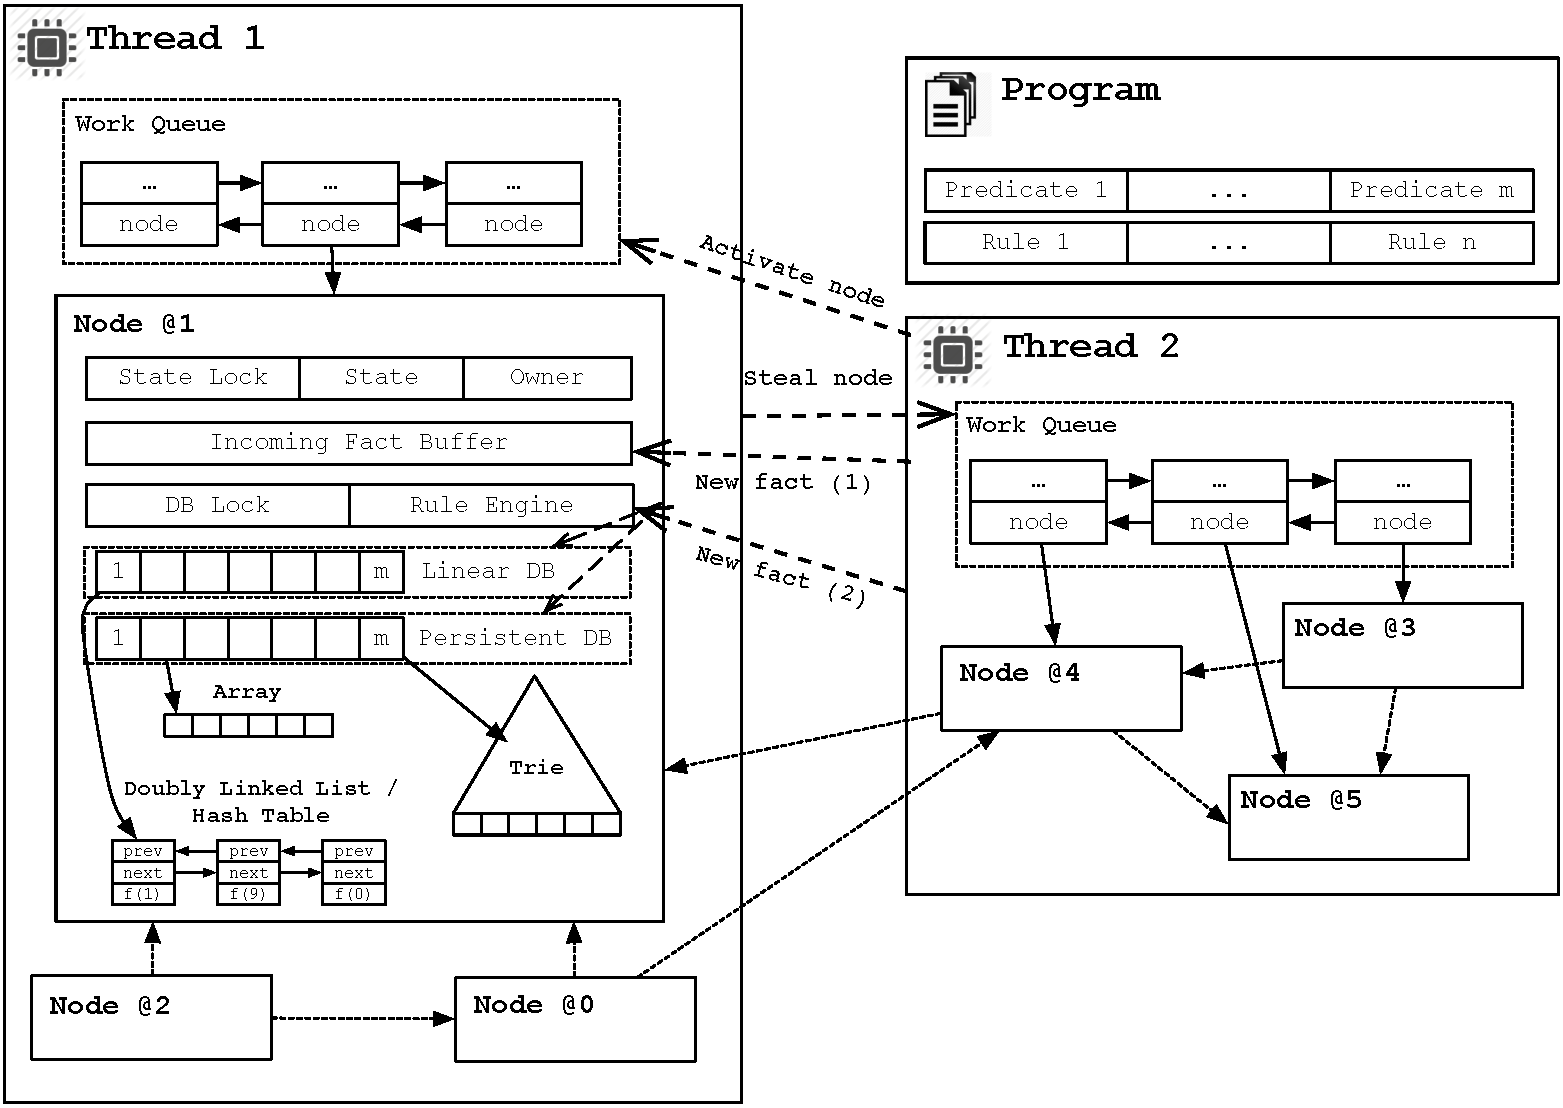
\includegraphics[width=\textwidth]{figures/implementation/vm_overview.pdf}
\caption{Layout of the virtual machine. Each thread has a work queue that
   contains active nodes (nodes with facts to process) that are processed one
   by one by the thread. Communication between threads happens when nodes
   send facts to nodes located in other threads.}
\label{fig:implementation:vm_overview}
\end{figure*}

Whenever a new fact is derived through rule derivation, we need to update the
data structures for the corresponding node. This is trivial if the thread that
derived the fact also owns the node. If that is not the case, then we have to
synchronize since multiple threads might be updating the same node's data
structures. We added a lock and a boolean flag to each node to protect the
access to its data structures. When the flag is activated, it means that the
node is currently being executed by the owning thread. For example, in
Fig.~\ref{fig:implementation:vm_overview}, if thread 2 derives a fact to node
\texttt{@1} (owned by thread 1), then thread 2 checks the node's flag and if not
activated, will lock node \texttt{@1} and perform the required updates
(\emph{New fact (1)}). If the flag is activated, it will not touch the main node
data structures, but instead will add the new fact to \emph{Fact Buffer}
(\emph{New fact (2)}). The facts stored in \emph{Fact Buffer} will then be
processed whenever the corresponding node's flag becomes active.

There is another thread interaction that might happen during fact derivation if
the node receiving a new fact is not active. In such case, the sending thread
needs to activate the node by pushing it to the \emph{Work Queue} of the target
thread. For example, consider again the situation in which thread 2 sends a new
fact to node \texttt{@1}. If node \texttt{@1} is not active, then thread 2 also
needs to activate it by pushing it to the \emph{Work Queue} of thread 1. After
this synchronization point, if the target thread is currently idle, it will
become active and with a new node to process.

\subsection{Runtime Data Structures And Garbage Collection}

LM also supports recursive types such as lists and pairs. These complex data
structures are stored in the heap of the VM and are managed through reference
counting. For instance, each list is a \emph{cons cell} with 3 fields:
\texttt{tail}, the pointer to the next element of the list; \texttt{head}, the
element stored by this element of the list; and \texttt{refs} that counts the
number of pointers to this list element in the VM. The list is deleted from the
heap whenever \texttt{refs} is decremented to zero.

Nodes are also subject to garbage collection. If the database of a node becomes
empty and there are no references to the node from other logical facts, then
the node is deleted from the program.

We avoid garbage collection schemes based on tracing since objects are created
and discarded in very specific points of the virtual machine and the runtime
objects cannot contain circular references. A reference counting mechanism is
thus more appropriate than a parallel tracing garbage collector which would
entail pausing the execution of the program to garbage collect all the unused
objects.

